\begin{framed}\noindent
	
	\textbf{Bài 2 - Bài toán đề nghị tháng 8/2018 - Nguyễn Hoàng Nam}
	
	Cho tam giác $\triangle ABC$ nội tiếp $(O)$. Trung trực $AB$ cắt đường tròn \textit{A-Apollonius} tại $H, I$ ($I$ gần $O$ hơn $H$). $K$ đối xứng với $I$ qua $BC$. Gọi $J = AK \cap CH$. Chứng minh rằng $JK$ là phân giác góc $\angle BJC$.
	
\end{framed}

\textbf{Lời giải 1 - Trần Quốc Thịnh.}

\begin{center}
	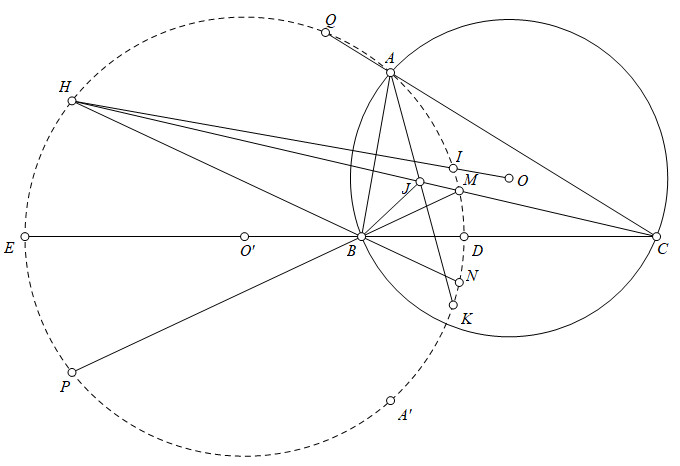
\includegraphics[scale=0.6]{T082018/T82018_NamNH_SOL1}
	
\end{center}

Gọi giao của $BC$ với đường tròn $A-Apollonius$ là $D$ và $E$ (điểm $D$ nằm giữa $B$ và $C$). Gọi $O'$ là tâm của đường tròn $A-Apollonis$, $A'$ là đối xứng của $A$ qua $BC$. Gọi $M$, $N$, $P$ và $Q$ lần lượt là giao của $CH$, $BH$, $BM$ và $CA$ với $(ADE)$ ta có: $\angle BO'Q = 2 \angle DEQ = 2 \angle CAD = \angle BAC$.

Suy ra tứ giác $ABO'Q$ nội tiếp, ta có:
$ CB . CO' = CA . CQ = CM . CH$.

Suy ra tứ giác $BMHO'$ nội tiếp, ta có: $ \angle NBD = \angle O'BH = \angle O'MH = \angle DBM$.

Vậy điểm $N$ đối xứng với điểm $M$ qua $BC$ nên điểm $P$ đối xứng với $H$ qua $BC$. Vậy góc $\angle MHA' = \angle AHN = 2\angle AHI = 2\angle KHA'$ nên $HK$ là phân giác góc $\angle MHA'$.

Vậy ta có: $KM = KA' = IA = IB = BK$.

Vậy tam giác $\triangle KBM$ cân tại $K$ nên ta có: $ \angle KJM = \angle JHK + \angle JKH = \angle IHA + \angle AIH = \angle HKI = \angle PIK = \angle PMK = \angle KBM$.

Vậy tứ giác $MJBK$ nội tiếp nên $JK$ là phân giác góc $\angle BJC$. $\qquad \blacksquare$

\textbf{Lời giải 2 - Đoàn Thành Đạt}

\textbf{Bổ đề 1.} Cho tam giác $\triangle ABC$, điểm $P$ bất kì. Chứng minh rằng điểm $P$ nằm trên đường tròn $A-Apollonius$ khi và chỉ khi: $\angle PAB + \angle PCB = \angle PAC + \angle PBC$.
\begin{center}
	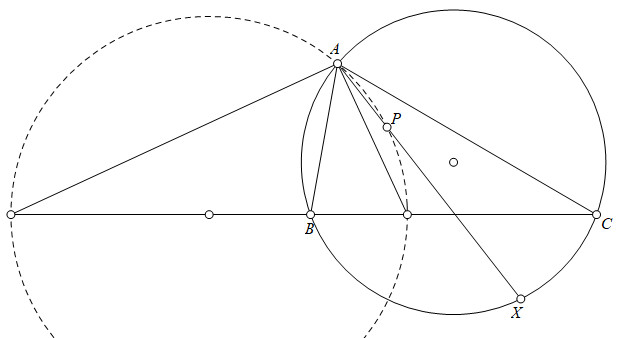
\includegraphics[scale=0.6]{T082018/T82018_NamNH_SOL2}
	
\end{center}

\textbf{Chứng minh bổ đề 1.}

\textit{Chiều đảo.}
Gọi $X = AP \cap (ABC)$ (điểm $X \neq A$) thì góc $\angle XBP = \angle PAB + \angle PCB = \angle PAC + \angle PBC = \angle XCP$. Suy ra:
\[
\frac{PB}{PC} = \frac{\sin(\angle PXB)}{\sin(\angle PXC)} = \frac{AB}{AC}
\]
Vậy điểm $P$ thuộc đường tròn $A-Apollonius$.

\textit{Chiều thuận.} Gọi hình chiếu của điểm $P$ lên $BC$, $AC$ và $AB$ lần lượt là $X$, $Y$ và $Z$. Thì ta có:
\[
\frac{PB}{PC} =\frac{AB}{AC} = \frac{\sin(\angle ACB)}{\sin(\angle ABC)}
\]
Vậy $XY = XZ$ suy ra $\angle PAB + \angle PCB = \angle PYZ + \angle PYX = \angle ZYX = \angle YZX = \angle PZY + \angle PZX = \angle PAC + \angle PBC$.

\textbf{Bổ đề 2.} Cho tam giác $\triangle ABC$ nội tiếp đường tròn $(O)$, trung trực $AB$ cắt đường tròn $A-Apollonius$ của tam giác $\triangle ABC$ tại $H$ và $I$ (điểm $I$ gần $O$ hơn $H$). Chứng minh rằng $CH$ và $CI$ đẳng giác trong góc $\angle BCA$.

\begin{center}
	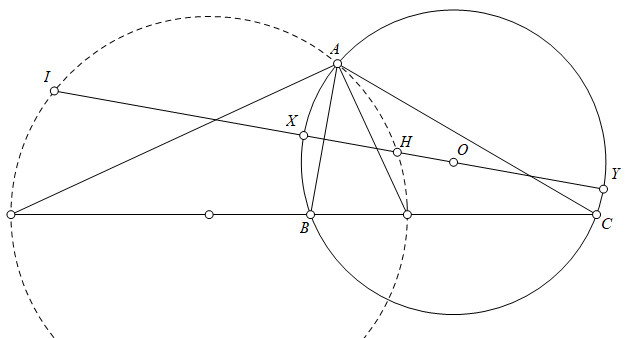
\includegraphics[scale=0.6]{T082018/T82018_NamNH_SOL3}
	
\end{center}

\textbf{Chứng minh bổ đề 2.}

Do đường tròn $A-Apollonius$ trực giao với $(O)$ nên $AO$ là tiếp tuyến của tam giác $\triangle HAI$. Vậy $(O)$ là đường tròn $A$-Apollonius của tam giác $\triangle HAI$.

Gọi giao của $HI$ với $(O)$ tại $X$ và $Y$ (điểm $X$ nằm giữa $H$ và $I$). Thì $(HI,XY) = -1$ mà góc $\angle XCY = 90$ nên $CX$ là phân giác góc $\angle ICH$. Vậy $CH$ và $CI$ đẳng giác trong góc $\angle BCA$.

\textbf{Quay lại bài toán.}

Gọi phân giác trong của góc $\angle BAC$ là $AD$, thì $D$ thuộc đường tròn $A-Apollonius$. Do $DI = DK$ nên $AD$ là phân giác góc $\angle IAK$ vậy $AI$ và $AJ$ đẳng giác trong góc $\angle BAC$.

Mà theo \textbf{Bổ đề 2} thì ta có $CI$ và $CH$ đẳng giác trong góc $\angle ACB$ nên điểm $I$ và $J$ liên hợp đẳng giác với nhau trong tam giác $\triangle ABC$.

Theo \textbf{Bổ đề 1} thì do điểm $I$ thuộc đường tròn $A-Apollonius$ của tam giác $\triangle ABC$ nên:
\[
\angle IAB + \angle ICB = \angle IAC + \angle IBC
\]
\[
\angle JAC + \angle JCA = \angle JAB + \angle JBA
\]
\[
\angle KJC = \angle KJB
\]
Vậy $JK$ là phân giác góc $\angle BAC$. $\qquad \blacksquare$

\underline{Nhận xét.} Lời giải của \textbf{Đoàn Thành Đạt} giống ý tưởng của tác giả dùng để sáng tác bài này. Còn lời giải của \textbf{Trần Quốc Thịnh} thì rõ ràng và ngắn gọn bằng cách sử dụng các cạnh bằng nhau để suy ra các cung bằng nhau. Ngoài ra thì bạn \textbf{Trần Quân} và \textbf{Nguyễn Hà An} cũng có những lời giải đúng với ý tưởng gần giống \textbf{Trần Quốc Thịnh}.

Ngoài ra ta cũng có tính chất như sau:

- Cho tam giác $\triangle ABC$, điểm $X$ bất kì nằm trên đường tròn $A$-Apollonius của tam giác $\triangle ABC$. Điểm đẳng giác của $X$ trong tam giác $\triangle ABC$ là $Y$. Chứng minh rằng $AY$ là phân giác góc $\angle BYC$.

- Cho tam giác $\triangle ABC$, điểm $X$ bất kì nằm trên đường tròn $A$-Apollonius của tam giác $\triangle ABC$. Gọi $Y$ là đối xứng của $X$ qua $BC$. Chứng minh rằng $AY$, $AX$ đẳng giác nhau trong góc $\angle BAC$. $\qquad \blacksquare$